\documentclass{article}
\usepackage[pdftex]{graphicx} %for embedding images
\usepackage{url} %for proper url entries
\usepackage[bookmarks, colorlinks=false, pdfborder={0 0 0}, pdftitle={Introduction to Machine Learning Midterm}, pdfauthor={Nhut-Nam Le}, pdfsubject={troduction to Machine Learning}, pdfkeywords={report, exercises}]{hyperref} %for creating links in the pdf version and other additional pdf attributes, no effect on the printed document
%\usepackage[final]{pdfpages} %for embedding another pdf, remove if not required
\usepackage[utf8]{vietnam}
\usepackage{float}
\usepackage{fancyhdr}
\usepackage[utf8]{inputenc}
\usepackage{pythonhighlight}
\usepackage[left=3cm, right=3cm, top=2cm, bottom=2cm]{geometry}
\usepackage{parskip}
\usepackage{tikz}
\usepackage{hyperref}
\usepackage[]{algorithm2e}
\usepackage[noend]{algpseudocode}
\usepackage{amsmath}
\usepackage{amsfonts}
\usepackage{listings}
\usepackage{color}

\definecolor{dkgreen}{rgb}{0,0.6,0}
\definecolor{gray}{rgb}{0.5,0.5,0.5}
\definecolor{mauve}{rgb}{0.58,0,0.82}

\newcommand\T{\rule{0pt}{2.6ex}}       % Top strut
\newcommand\B{\rule[-1.2ex]{0pt}{0pt}} % Bottom strut


\newcommand{\foo}{\hspace{-2.3pt}$\bullet$ \hspace{5pt}}


\lstset{frame=tb,
	language=Java,
	aboveskip=3mm,
	belowskip=3mm,
	showstringspaces=false,
	columns=flexible,
	basicstyle={\small\ttfamily},
	numbers=none,
	numberstyle=\tiny\color{gray},
	keywordstyle=\color{blue},
	commentstyle=\color{dkgreen},
	stringstyle=\color{mauve},
	breaklines=true,
	breakatwhitespace=true,
	tabsize=3
}

\setlength{\parindent}{15pt}
\setlength{\headheight}{15.2pt}
\pagestyle{fancy}
\lhead[<even output>]{NHẬP MÔN HỌC MÁY}
\rhead[<even output>]{BÁO CÁO CUỐI KỲ}
\title{research-outline}
\author{Nhut-Nam Le}
\date{2021}

\begin{document}
	\begin{titlepage}
		\begin{center}
			% Top of the page
			\large{\textbf{ĐẠI HỌC KHOA HỌC TỰ NHIÊN, ĐHQG-HCM\\KHOA CÔNG NGHỆ THÔNG TIN\\BỘ MÔN KHOA HỌC MÁY TÍNH}}\\
			
\includegraphics[width=0.75\textwidth]{images/khtn.png}\\
			% Title
			\large \textbf{NHẬP MÔN HỌC MÁY}\\[0.1in]
			\huge \textbf{BÁO CÁO ĐỒ ÁN CUỐI KỲ}\\[0.1in]
			\huge \textbf{TÌM HIỂU: NHẬN DẠNG GIỌNG NÓI BẰNG SÓNG ÂM THÔ VỚI SINCNET}\\[0.1in]
			\vfill
			\normalsize
			\normalsize
			% Lecturers
			\textbf{Giảng viên lý thuyết}\\
			{\textbf{TS.} Bùi Tiến Lên}\\[0.1in]
			% Teacher Assistant
			\textbf{Giảng viên hướng dẫn}\\
			\vspace{0.1in}
			{Dương Nguyễn Thái Bảo, Nguyễn Ngọc Đức, Nguyễn Tiến Huy, Lê Thanh Phong}\\[0.1in]
			\textbf{Sinh viên thực hiện} \\
			\vspace{0.1in}
			% Submitted by
			{Vương Gia Bảo, Ngô Xuân Kiên, Lê Nhựt Nam, Nguyễn Viết Dũng}\\[0.1in]
			% Date time when written report
			\vfill
			Tháng 4 năm 2021
		\end{center}
	\end{titlepage}
	\newpage
	% End Title4
	
	\pagenumbering{roman} %numbering before main content starts
	\cleardoublepage
	%\pagebreak
	\phantomsection
	\addcontentsline{toc}{section}{Lời cảm ơn}
	\section*{Lời cảm ơn}
	\vspace{1.0in}
	\begingroup
	\setlength{\parindent}{0pt}
	\qquad Trong quá trình thực hiện đồ án này, chúng em đã nhận được rất nhiều sự giúp đỡ cũng như hỗ trợ từ các thầy cô Trường Đại học Khoa học Tự nhiên, ĐHQG-HCM và các bạn bè trong lớp Nhập môn Học Máy. Chúng em xin bày tỏ lòng cảm ơn chân thành đến mọi người vì đã giúp đỡ hướng dẫn, chỉ bảo rất tận tình.
	
	\qquad Đặc biệt, chúng em xin bày tỏ lòng biết ơn sâu sắc đến các thầy cô khoa Công nghệ Thông tin, cụ thể hơn là thầy Bùi Tiến Lên và các thầy hướng dẫn đã giảng dạy rất nhiệt, cung cấp nhiều slides, tài nguyên học tập cần thiết, tạo điều kiện tốt nhất để chúng em có thể hoàn thành được đồ án này.
	
	\qquad Trong quá trình, viết báo cáo này, chúng em không thể tránh khỏi nhiều thiếu sót, hy vọng mong nhận được góp ý từ thầy để chúng em tiếp tục hoàn thiện hơn đối với đồ án này, cũng như rút kinh nghiệm cho những đồ án, những báo cáo kế tiếp.
		
	\vspace{1.0in}
	\textbf{Đại học Khoa học Tự nhiên, ĐHQG-HCM.}\\
	Vương Gia Bảo, Ngô Xuân Kiên, Lê Nhựt Nam, Nguyễn Viết Dũng\\
	Tháng 4 năm 2021\\
	\endgroup
	
	\newpage
	\tableofcontents
	\newpage
	\pagenumbering{arabic} %reset numbering to normal for the main content
	\setcounter{secnumdepth}{0}
	
	\section{1. Đặt vấn đề}
	\qquad Trong những năm gần đây, Machine Learning (Học máy/ Máy học) đạt được rất nhiều thành tựu nổi bật, thúc đẩy Cách mạng Công nghệ 4.0 phát triển nhanh chóng. Một trong những tác nhân chính mạnh mẽ nhất đến từ Deep Learning (Deep Neural Networks - Các mạng Học sâu), các mô hình học dựa trên những phương pháp này đã rất thành công, đạt được một hiệu năng đầy triển vọng, trong nhiều tác vụ khác nhau như Thị giác Máy tính (Computer Vision), Nhận dạng Nhân trắc học (Biometrics): Giọng nói (Speech), Khuôn mặt (Face), Vân tay (Fingerprint), ..., Xử lý ngôn ngữ tự nhiên (Natural Language Processing), ...
	
	Trong tác vụ nhận dạng, đặc biệt là nhận dạng giọng nói (Voice/ Speech Recognition) gần như là một bài toán khó trong nhiều năm, cần những phương pháp rất phức tạp để có thể giải quyết được. Nhờ vào Học sâu, phương giải phải khả thi, mà cụ thể là với Mạng Neural Tích chập (Convolutional Neural Networks - CNNs) đem lại những kết quả đầy hứa hẹn khi chỉ cần đầu vào trực tiếp là mẫu giọng nói thô. Thay vì sử dụng các tính năng thủ công tiêu chuẩn, CNNs sau này học cách biểu diễn giọng nói cấp thấp từ các dạng sóng, có khả năng cho phép mạng nắm bắt tốt hơn các đặc điểm giọng nói ở dải tần hẹp quan trọng như cao độ và hình dạng.
	
	Với mục đích tìm hiểu bài báo khoa học, cũng như tìm hiểu những mô hình, phương pháp Học máy nổi bật gần đây trong những tác vụ quan trọng, mà cụ thể là nhận dạng. Nhóm chúng em quyết định chọn một bài báo khoa học liên quan đến Nhận dạng giọng nói và cũng là tài liệu nghiên cứu chính thực hiện chính cho đồ án môn học.
	
	\section{1. Giới thiệu}
	\qquad Phần tiếp nối công việc giữa kỳ, trong phần này nhóm trình bày cách xây dựng một Speaker Recognition Pipeline cơ bản: Chuẩn bị dữ liệu (Data preparation), Xây dựng phát triển mô hình (Development), Đăng ký (Enrollment), Đánh giá (Evaluation)
	
	\section{2. Chuẩn bị dữ liệu}
	\subsection{Dữ liệu giọng nói tiếng Anh}
	\qquad \textbf{Tiếng Anh} Sử dụng hai tập dữ liệu đã được đề cập trong bài báo
	
	Với \textbf{TIMIT}, ta có một kho ngữ liệu với 462 người nói, các khoảng không phải lời nói ở đầu và cuối mỗi câu đã bị xóa, những tập tin về nội dung câu nói của TIMIT cũng được loại bỏ. Sau khi tinh chỉnh toàn bộ dữ liệu, tác giả dùng 5 câu nói của mỗi người nói để huấn luyện, 3 câu nói của mỗi người nói dùng để kiểm tra.
	
	Với tập ngữ liệu \textbf{LibriSpeech}, những phần với độ im lặng bên trong kéo dài hơn 125 ms được chia thành nhiều phần nhỏ. Việc chia tập huấn luyện (training set), tập kiểm tra (testing set) là ngẫu nhiên bằng cách chọn 12-15 giây dữ liệu huấn luyện của mỗi người nói và các câu kiểm tra kéo dài từ 2-6 giây. 
	\subsection{Dữ liệu giọng nói tiếng Việt}
	Sử dụng tập dữ liệu Son et al. Dataset
	
	Nguồn dữ liệu từ bài báo Vietnamese Speaker Authentication Using Deep Models
	\begin{itemize}
		\item Dung lượng của tập dữ liệu: 535 MB
		\item Số mẫu trong tập dữ liệu: 400 mẫu
		\item Bộ dữ liệu gồm: hai tập  Men và Women, mỗi tập con chứa 10 thư mục người nói. Mỗi thư mục người nói chứa 20 đoạn ghi âm, chia ra Long và Short (mỗi loại 10 đoạn) 
		\item Nội dung câu nói
		\begin{itemize}
			\item Câu ngắn: “Tôi là sinh viên chuyên ngành công nghệ thông tin"
			\item Câu dài: "Tôi là sinh viên Học viện Công nghệ Bưu chính Viễn thông, chương trình đào tạo khá nặng đòi hỏi sinh viên phải học tập và nghiên cứu rất nhiều nhưng tôi tự hào vì đó là ngành đã và đang làm thay đổi cuộc sống xã hội loài người".
		\end{itemize}
		\item Điểm hạn chế: Bộ dữ liệu có kích thước khá nhỏ
	\end{itemize}
	
	Ngoài ra, nhóm tự ghi âm thêm dữ liệu với độ dài tương tự như tập này.
	
	\section{3. Xây dựng thực nghiệm}
	\subsection{Thực nghiệm trên tập TIMIT}
	\begin{itemize}
		\item Xử lý dữ liệu
		\item Mô hình 
		\begin{itemize}
			\item Các cửa sổ có $\text{fs} = 16000$, tín hiệu được cắt thành những chunks với $\text{cw\_len}=200$, overlap $\text{cw\_shift}=10$s
			\item Lớp Input: sử dụng 80 bộ lọc SincNet có kích thước $L=251$, max pool - 3, sử dụng Layer Norm cho cả input và output, không dùng Batch Norm, hàm kích hoạt activation leaky-ReLU, dropout = 0
			\item Hai lớp CNN: sử dụng 2 lớp CNN, với mỗi lớp dùng 60 bộ lọc có kích thuốc $L=5$, sử dụng Layer Norm cho cả input và output, không dùng Batch Norm, hàm kích hoạt activation leaky-ReLU, dropout = 0
			\item Ba lớp DNN: sử dụng 3 lớp DNN (Multi Layer Perceptron) fully-connected với 2048 neurons, Layer Norm cho input, Batch Norm cho output, các lớp ẩn (hidden layers) dùng leaky-ReLU
			\item Lớp Output: Multi Layer Perceptron, 462 nodes, không dropout, không LayerNorm, không BatchNorm cho cả input và output, hàm activation function dùng softmax
			\item Hàm mất mát: Negative Log Likelihood Loss
		\end{itemize}
		\item Hyper parameters
		\begin{itemize}
			\item learning rate $\text{lr} = 0.001$
			\item $\alpha = 0.95$
			\item $\epsilon = 10^{-7}$
			\item $\text{batch\_size}=128$
			\item $\text{N\_epochs}=100$
			\item $\text{N\_batches}=800$
			\item $\text{N\_eval\_epoch}=8$
			\item $\text{seed}=1234$
		\end{itemize}
	\end{itemize}
	\subsection{Thực nghiệm trên tập Librispeech}
	\begin{itemize}
		\item Xử lý dữ liệu
		\item Mô hình 
		\begin{itemize}
			\item Các cửa sổ có $\text{fs} = 8000$, tín hiệu được cắt thành những chunks với $\text{cw\_len}=375$, overlap $\text{cw\_shift}=10$s
			\item Lớp Input: sử dụng 80 bộ lọc SincNet có kích thước $L=251$, max pool - 3, sử dụng Layer Norm cho cả input và output, không dùng Batch Norm, hàm kích hoạt activation leaky-ReLU, dropout = 0
			\item Hai lớp CNN: sử dụng 2 lớp CNN, với mỗi lớp dùng 60 bộ lọc có kích thuốc $L=5$, sử dụng Layer Norm cho cả input và output, không dùng Batch Norm, hàm kích hoạt activation leaky-ReLU, dropout = 0
			\item Hai lớp DNN: sử dụng 2 lớp DNN (Multi Layer Perceptron) fully-connected với 2048 neurons, Layer Norm cho input, Batch Norm cho output, các lớp ẩn (hidden layers) dùng leaky-ReLU làm activation cho lớp DNN thứ nhất, lớp kia dùng linear
			\item Lớp Output: 2 lớp Multi Layer Perceptron, 2048 nodes cho mỗi lớp, không dropout, Layer Norm cho input, Batch Norm cho output, hàm activation function lớp thứ nhất dùng leaky-ReLU, lớp thứ hai dùng softmax
			\item Hàm mất mát: Negative Log Likelihood Loss
		\end{itemize}
		\item Hyper parameters
		\begin{itemize}
			\item learning rate $\text{lr} = 0.001$
			\item $\alpha = 0.95$
			\item $\epsilon = 10^{-7}$
			\item $\text{batch\_size}=128$
			\item $\text{N\_epochs}=100$
			\item $\text{N\_batches}=100$
			\item $\text{N\_eval\_epoch}=10$
			\item $\text{reg\_factor}=1000$
			\item $\text{fact\_amp=0.2}$
			\item $\text{seed}=1234$
		\end{itemize}
	\end{itemize}
	\subsection{Thực nghiệm trên tập Son et al. Dataset}
	\begin{itemize}
		\item Xử lý dữ liệu
		\item Mô hình 
		\begin{itemize}
			\item Các cửa sổ có $\text{fs} = 16000$, tín hiệu được cắt thành những chunks với $\text{cw\_len}=200$, overlap $\text{cw\_shift}=10$s
			\item Lớp Input: sử dụng 80 bộ lọc SincNet có kích thước $L=251$, max pool - 3, sử dụng Layer Norm cho cả input và output, không dùng Batch Norm, hàm kích hoạt activation leaky-ReLU, dropout = 0
			\item Hai lớp CNN: sử dụng 2 lớp CNN, với mỗi lớp dùng 60 bộ lọc có kích thuốc $L=5$, sử dụng Layer Norm cho cả input và output, không dùng Batch Norm, hàm kích hoạt activation leaky-ReLU, dropout = 0
			\item Ba lớp DNN: sử dụng 3 lớp DNN (Multi Layer Perceptron) fully-connected với 2048 neurons, Layer Norm cho input, Batch Norm cho output, các lớp ẩn (hidden layers) dùng leaky-ReLU
			\item Lớp Output: Multi Layer Perceptron, 18 nodes, không dropout, không LayerNorm, không BatchNorm cho cả input và output, hàm activation function dùng softmax
			\item Hàm mất mát: Negative Log Likelihood Loss
		\end{itemize}
		\item Hyper parameters
		\begin{itemize}
			\item learning rate $\text{lr} = 0.001$
			\item $\alpha = 0.95$
			\item $\epsilon = 10^{-7}$
			\item $\text{batch\_size}=128$
			\item $\text{N\_epochs}=300$
			\item $\text{N\_batches}=100$
			\item $\text{N\_eval\_epoch}=1$
			\item $\text{seed}=1234$
		\end{itemize}
	\end{itemize}
	\section{4. Đăng ký}
	
	\section{5. Đánh giá mô hình}
	\subsection{Kết quả thực nghiệm trên tập TIMIT}
	Các kết quả khi đánh giá mô hình bằng tập TIMIT
	\begin{figure}[H]
		\centering
		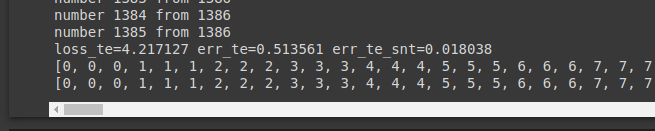
\includegraphics[width=.75\textwidth]{result/evaluate_result_timit.png}
		\caption{Kết quả thực nghiệm trên TIMIT Dataset}
		\label{fig:writing-thesis}
	\end{figure}
	\begin{itemize}
		\item Độ lỗi huấn luyện trung bình mỗi frame $loss\_tr=4.217127$
		\item Giá trị phân lớp sai mức frame $err\_te=0.513561$
		\item Giá trị phân lớp sai mức câu $err\_te\_snt =0.018038$
	\end{itemize}
	\begin{figure}[H]
		\centering
		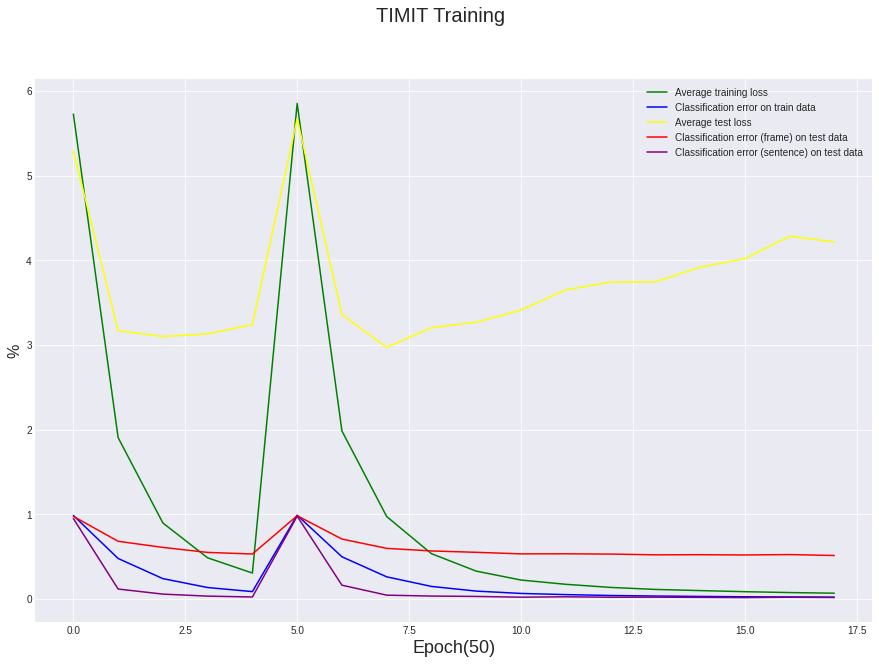
\includegraphics[width=.75\textwidth]{result/sincnet_timit_plot.png}
		\caption{Kết quả thực nghiệm trên TIMIT Dataset}
		\label{fig:writing-thesis}
	\end{figure}
	\subsection{Kết quả thực nghiệm trên tập Librispeech}
	Các kết quả khi đánh giá mô hình bằng tập Librispeech
	\begin{figure}[H]
		\centering
		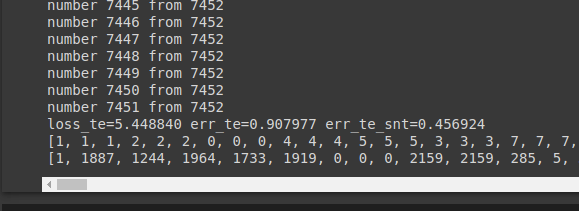
\includegraphics[width=.75\textwidth]{result/evaluate_result_libris.png}
		\caption{Kết quả thực nghiệm trên Librispeech Dataset}
		\label{fig:writing-thesis}
	\end{figure}
	\begin{itemize}
		\item Độ lỗi huấn luyện trung bình mỗi frame $loss\_tr=5.448840$
		\item Giá trị phân lớp sai mức frame $err\_te=0.907977$
		\item Giá trị phân lớp sai mức câu $err\_te\_snt =0.456924$
	\end{itemize}
	\begin{figure}[H]
		\centering
		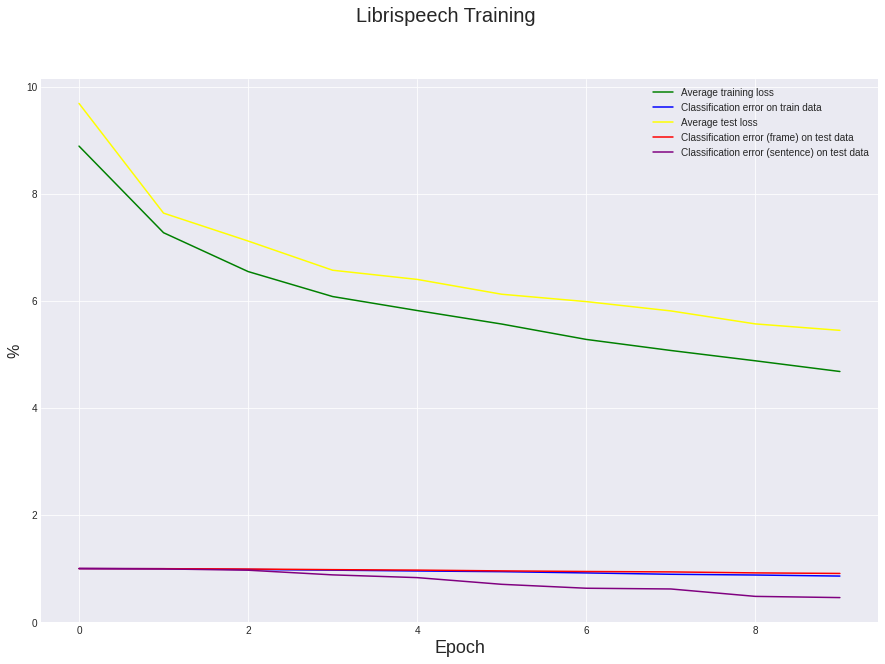
\includegraphics[width=.75\textwidth]{result/sincnet_librispeech_plot.png}
		\caption{Kết quả thực nghiệm trên Librispeech Dataset}
		\label{fig:writing-thesis}
	\end{figure}
	\subsection{Kết quả thực nghiệm trên tập Son et al. Dataset}
	Các kết quả khi đánh giá mô hình bằng tập Son et al. Dataset
	\begin{figure}[H]
		\centering
		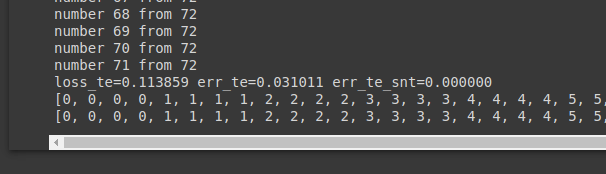
\includegraphics[width=.75\textwidth]{result/evaluate_result_vn_speaker.png}
		\caption{Kết quả thực nghiệm trên Son et al. Dataset}
		\label{fig:writing-thesis}
	\end{figure}
	\begin{itemize}
		\item Độ lỗi huấn luyện trung bình mỗi frame $loss\_tr=0.113859$
		\item Giá trị phân lớp sai mức frame $err\_te=0.031011$
		\item Giá trị phân lớp sai mức câu $err\_te\_snt =0.000000$
	\end{itemize}
	\begin{figure}[H]
		\centering
		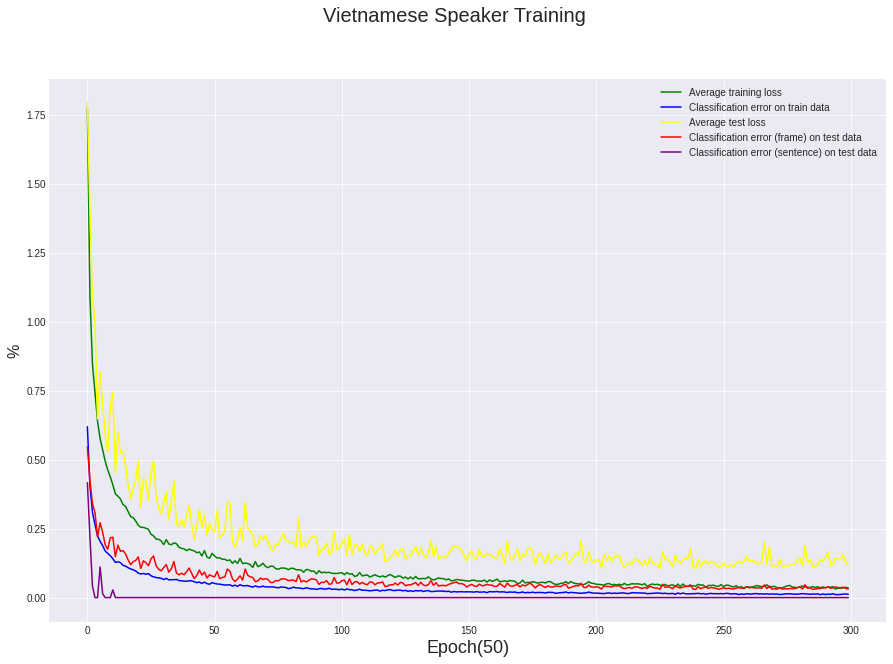
\includegraphics[width=.75\textwidth]{result/sincnet_vietnamese_plot.png}
		\caption{Kết quả thực nghiệm trên Son et al. Dataset}
		\label{fig:writing-thesis}
	\end{figure}
	\section{6. Kết luận}
	
	\section{7. Kế hoạch thực hiện}
	
	\subsection{7.1 Timeline}
	\scalebox{1}{
		\begin{tabular}{r |@{\foo} l}
			
			29/03 - 04/04 & Tiếp nhận đồ án, phân công công việc\\
			05/04 - 11/04 & Đọc source code mẫu từ Github, trình bày những gì tìm hiểu được\\
			12/04 - 18/04 & Chạy thử source code mẫu từ Github, trình bày những gì tìm hiểu được\\
			19/04 - 25/04 & Trình bày những gì tìm hiểu được, phân công làm slides, quay video trình bày đồ án\\
			26/04 - 02/05 & Thu thập dữ liệu, tiền xử lý dữ liệu\\
			03/05 - 09/05 & Tinh chỉnh source code, chạy thử mô hình\\
			10/05 - 16/05 & Huấn luyện mô hình\\
			17/05 - 23/05 & Phân công làm slides, quay video trình bày đồ án\\
			24/05 - 30/05 & *Dự phòng\\
			31/05 - 06/06 & *Dự phòng\\
			
		\end{tabular}
	}
	
	\subsection{7.2 Vai trò của các thành viên}
	\begin{table}[H]
		\centering
		\begin{tabular}{ | p{1cm} |  p{3cm} | p{5cm} | p{5cm}  |}\hline
			STT	& MSSV & Họ tên đầy đủ & Email liên lạc \\\hline
			1 & 18120009 & Vương Gia Bảo & 18120009@student.hcmus.edu.vn  \\ \hline
			2 & 18120045 & Ngô Xuân Kiên & 18120045@student.hcmus.edu.vn \\ \hline
			3 & 18120061 & Lê Nhựt Nam (Nhóm trưởng)& 18120061@student.hcmus.edu.vn  \\ \hline
			4 & 18120167 & Nguyễn Viết Dũng &  18120167@student.hcmus.edu.vn \\ \hline
		\end{tabular}
	\end{table}
	
	\subsection{7.3 Phân công công việc}
	\begin{table}[H]
		\begin{tabular}{ | l | l | l | p{5.5cm} | p{3cm} |}
			\hline
			STT & MSSV & Họ tên & Nội dung công việc & Mức độ hoàn thành  \\ \hline
			1 & 18120009 & Vương Gia Bảo & Thu thập dữ liệu, đọc hiểu source, báo cáo Introduction Paper &  100\%\T\B\\ \hline
			2 & 18120045 & Ngô Xuân Kiên & Thu thập dữ liệu, đọc hiểu source, báo cáo Related Work Paper & 100\%\T\B \\ \hline
			3 & 18120061 & Lê Nhựt Nam & Thu thập dữ liệu, đọc hiểu source, báo cáo, SincNet Architecture, Slides thuyết trình, Midterm Report & 100\%\T\B \\ \hline
			4 & 18120167 & Nguyễn Viết Dũng &  Thu thập dữ liệu, đọc hiểu source, báo cáo experimental setup Paper & 100\%\T\B \\ \hline
		\end{tabular}
	\end{table}
	\nocite{*}
	\bibliography{references}\newpage\cleardoublepage
	\bibliographystyle{plain}
	

\end{document}